\documentclass[12pt]{article}
\usepackage{hyperref}
\usepackage{listings}
\usepackage[margin=1in]{geometry}
\usepackage{enumitem}
\usepackage{multicol}
\usepackage{array}
\usepackage{titlesec}
\usepackage{helvet}
\renewcommand{\familydefault}{\sfdefault}
\usepackage{amsmath}     % For math equations
\usepackage{amssymb}     % For advanced math symbols
\usepackage{amsfonts} % For math fonts
\usepackage{gvv}
\usepackage{esint}
\usepackage[utf8]{inputenc}
\usepackage{graphicx}
\usepackage{pgfplots}
\pgfplotsset{compat=1.18}
\titleformat{\section}{\bfseries\large}{\thesection.}{1em}{}
\setlength{\parindent}{0pt}
\setlength{\parskip}{6pt}
\usepackage{multirow}
\usepackage{float}
\usepackage{caption}


\begin{document}

\section*{Problem 12.318}
Let $V$ be the vector space of all real polynomials of degree at most $20$. 
Define the subspaces
\begin{align}
W_1 = \{ p \in V : p(1)=p(\tfrac12)=p(5)=p(7)=0 \}, \quad 
W_2 = \{ p \in V : p(\tfrac12)=p(3)=p(4)=p(7)=0 \}.
\end{align}
Find $\dim(W_1 \cap W_2)$ .

\section*{Input Variables}
\begin{table}[H]
\centering
\begin{tabular}{|c|c|}
\hline
Symbol & Description \\
\hline
$p(x)$ & Polynomial of degree $\leq 20$ \\
$c_i$ & Coefficients of $p(x)$ \\
$a$ & Point of evaluation (root condition) \\
$A$ & Constraint matrix from evaluations \\
\hline
\end{tabular}
\caption{} \label{}
\end{table}

\section*{Definitions}

\textbf{Vector Space:}  
A set $V$ together with two operations (vector addition and scalar multiplication) is called a vector space over the field $\mathbb{R}$ if for all $\vec{u},\vec{v},\vec{w} \in V$ and scalars $a,b \in \mathbb{R}$, the following conditions hold:
\begin{itemize}
    \item Closure under addition: $\vec{u}+\vec{v} \in V$.
    \item Commutativity: $\vec{u}+\vec{v} = \vec{v}+\vec{u}$.
    \item Associativity: $(\vec{u}+\vec{v})+\vec{w} = \vec{u}+(\vec{v}+\vec{w})$.
    \item Existence of zero vector: $\exists \, \vec{0} \in V$ such that $\vec{u}+\vec{0}=\vec{u}$.
    \item Existence of additive inverse: $\forall \vec{u}\in V, \, \exists (-\vec{u}) \in V$ such that $\vec{u}+(-\vec{u})=\vec{0}$.
    \item Closure under scalar multiplication: $a\vec{u} \in V$.
    \item Distributivity: $a(\vec{u}+\vec{v}) = a\vec{u}+a\vec{v}$ and $(a+b)\vec{u}=a\vec{u}+b\vec{u}$.
    \item Compatibility: $a(b\vec{u})=(ab)\vec{u}$.
    \item Identity: $1\cdot \vec{u}=\vec{u}$.
\end{itemize}

\textbf{Subspace:}  
A subset $W \subseteq V$ is called a subspace of $V$ if:
\begin{enumerate}
    \item $\vec{0} \in W$ (contains the zero vector),
    \item If $\vec{u},\vec{v}\in W$, then $\vec{u}+\vec{v}\in W$ (closed under addition),
    \item If $\vec{u}\in W$ and $\alpha \in \mathbb{R}$, then $\alpha \vec{u} \in W$ (closed under scalar multiplication).
\end{enumerate}

\textbf{Dimension of a Subspace:}  
The dimension of a subspace $W$ of $V$ is the number of vectors in a basis of $W$, i.e.,
\[
\dim(W) = \text{number of linearly independent vectors that span } W.
\]

\section*{Solution}

\noindent
Step 1: Represent the polynomial
\begin{align}
p(x) &= c_0 + c_1x + c_2x^2 + \cdots + c_{20}x^{20}, \\
\vec{c} &= \myvec{c_0 \\ c_1 \\ \vdots \\ c_{20}} \in \mathbb{R}^{21}.
\end{align}

\noindent
Step 2: Each condition $p(a)=0$ gives
\begin{align}
p(a) &= \myvec{1 & a & a^2 & \cdots & a^{20}} \vec{c} = 0.
\end{align}

\noindent
Step 3: For the intersection $W_1 \cap W_2$, the polynomial must vanish at 
\[
\{1,\tfrac12,5,7,3,4\}.
\]
Thus we obtain the matrix equation
\begin{align}
A \vec{c} &= \vec{0}, \quad \text{where} \\
A &= \myvec{
1 & 1 & 1^2 & \cdots & 1^{20} \\
1 & \tfrac12 & (\tfrac12)^2 & \cdots & (\tfrac12)^{20} \\
1 & 5 & 5^2 & \cdots & 5^{20} \\
1 & 7 & 7^2 & \cdots & 7^{20} \\
1 & 3 & 3^2 & \cdots & 3^{20} \\
1 & 4 & 4^2 & \cdots & 4^{20}
}.
\end{align}

\noindent
Step 4: The system $A\vec{c}=\vec{0}$ is a homogeneous system with $21$ unknowns 
and $6$ independent equations. Hence the number of free variables is
\begin{align}
21 - 6 = 15.
\end{align}

\noindent
\textbf{Final Answer:}
\begin{align}
\dim(W_1 \cap W_2) = 15
\end{align}

\begin{figure}[H]
    \centering
    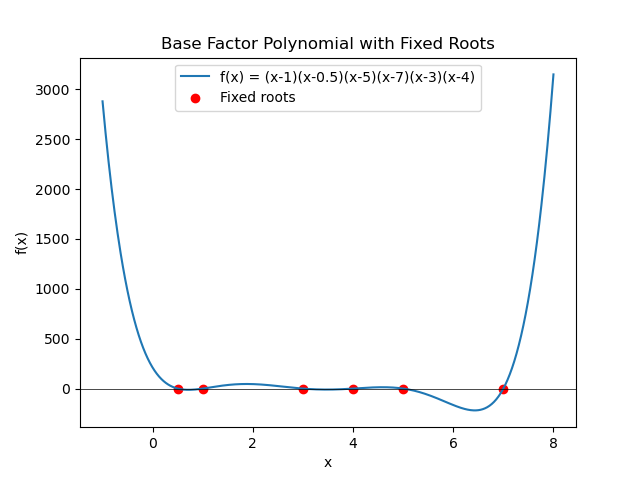
\includegraphics[width=0.9\columnwidth]{figs/poly_dim.png}
    \caption{}
    \label{fig:placeholder}
\end{figure}

\end{document}
